\documentclass[11pt,a4paper]{article}
\usepackage[utf8]{inputenc}
\usepackage[T1]{fontenc}
\usepackage{lmodern}
\usepackage[a4paper,margin=2.2cm,top=2.2cm,bottom=2.2cm]{geometry}
\usepackage{xcolor}
  \definecolor{accent1}{HTML}{B45309}
  \definecolor{accent2}{HTML}{075985}
  \definecolor{accent3}{HTML}{166534}
  \definecolor{accent4}{HTML}{6B21A8}
  \definecolor{accent5}{HTML}{B91C1C}
\usepackage[colorlinks=true,linkcolor=blue,urlcolor=blue,citecolor=blue]{hyperref}
\usepackage{amsmath,amssymb,amsthm}
\usepackage{booktabs}
\usepackage{array}
\usepackage{tikz}
  \usetikzlibrary{positioning,arrows.meta,shapes.geometric,fit,backgrounds,calc,decorations.pathmorphing}
\usepackage{fancyhdr}
  \pagestyle{fancy}
  \fancyhf{}
  \fancyhead[L]{Differential Geometry on Signed Hypergraphs}
  \fancyhead[R]{Primer for G\"ombSoma}
  \fancyfoot[C]{\thepage}

\setlength{\parskip}{0.55em}
\setlength{\parindent}{0pt}

\newtheorem{theorem}{Theorem}[section]
\newtheorem{proposition}[theorem]{Proposition}
\newtheorem{definition}[theorem]{Definition}
\newtheorem{remark}[theorem]{Remark}

\newcommand{\sig}{\ensuremath{\sigma}}

\title{Differential Geometry on Signed Hypergraphs \\
       \large{A primer for the G\"ombSoma--Ricci-Stim architecture}}
\date{2026-05-14}
\author{}

\begin{document}

\maketitle
\thispagestyle{fancy}

\begin{abstract}
\noindent This primer collects, in roughly the order they appear in the
G\"ombSoma--Ricci-Stim plan, the differential-geometric machinery that
makes ``hypergraph convolution'' a principled object rather than an
ad-hoc message-passing rule. We cover: simplicial complexes and signed
boundary operators; the Hodge Laplacian at each simplex dimension; the
Hodge decomposition theorem; the heat kernel; Forman-Ricci and
Ollivier-Ricci curvature; the Bochner--Weitzenböck identity that
couples curvature to the Laplacian; and discrete Ricci flow as a
graph-rewiring tool. Each section has a small example, a TikZ figure,
and a one-line takeaway for how the concept enters the architecture.
\end{abstract}

\section{Why bother}

A standard CNN is a discretisation of the heat equation
$\partial_t u = \Delta u$ on a planar grid: the convolution kernel is a
finite-difference Laplacian, ReLU is a flow-rectifier, pooling is a
local average. The whole CNN stack is a clumsy approximation of a
continuous geometric process.

\emph{Hypergraph} networks generalise this to irregular topology
($V, E$ instead of an $H \times W$ grid). \emph{Signed} hypergraphs
generalise further: edges carry a sign $\sig(e) \in \{-1, +1\}$
encoding polarity (trust / distrust, rotational / prismatic,
brightness-up / brightness-down). The full Riemannian-geometric stack
--- boundary operators, Laplacians, curvature, heat flow, Bochner
identities --- transfers across these generalisations almost verbatim.
This primer makes that transfer explicit.

The one-sentence takeaway: \emph{the architecture we want to build is
the natural discretisation of Riemannian geometry on a signed
simplicial complex}. Forman gave us Ricci curvature
\cite{Forman2003}; Topping et al.\ gave us the over-squashing diagnosis
\cite{Topping2022}; Cartwright \& Harary gave us the signed-balance
theory \cite{Cartwright1956}. The architecture is what happens when you
put them in the same box.

\section{Simplicial complexes}

\begin{definition}[Simplicial complex]
A finite collection $K$ of finite subsets of a vertex set $V$, closed
under taking subsets: if $\sigma \in K$ and $\tau \subseteq \sigma$,
then $\tau \in K$. Elements of $K$ are called \emph{simplices}; a
simplex of size $k+1$ is a $k$-\emph{simplex}.
\end{definition}

The $0$-simplices are vertices; $1$-simplices are edges; $2$-simplices
are (filled) triangles; $3$-simplices are tetrahedra; and so on. A
signed hypergraph $H = (V, E, \sig)$ presents the data of a signed
simplicial complex if we additionally include the triangles (and
higher) determined by the $\sig$-product structure.

\begin{center}
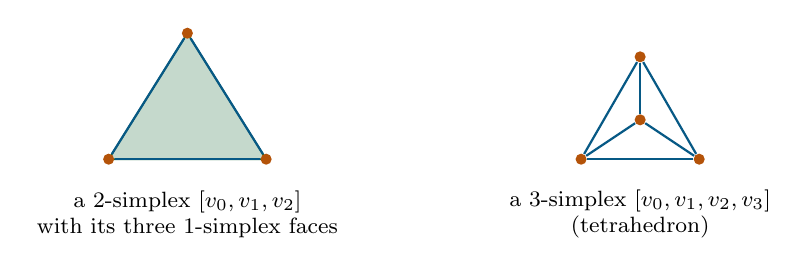
\begin{tikzpicture}[scale=1.0,
    vertex/.style={circle, fill=accent1, inner sep=0pt,
                   minimum size=4pt, label/.style={font=\footnotesize}},
    edge/.style={draw=accent2, line width=0.8pt},
    face/.style={fill=accent3!25, draw=accent3, line width=0.6pt}]
  % 2-simplex (triangle) with edges and vertices
  \fill[face] (0,0) -- (2,0) -- (1, 1.6) -- cycle;
  \node[vertex, label=below left:{$v_0$}] (a) at (0,0) {};
  \node[vertex, label=below right:{$v_1$}] (b) at (2,0) {};
  \node[vertex, label=above:{$v_2$}] (c) at (1, 1.6) {};
  \draw[edge] (a) -- (b);
  \draw[edge] (b) -- (c);
  \draw[edge] (a) -- (c);
  \node[font=\footnotesize, align=center] at (1, -0.7) {a $2$-simplex $[v_0, v_1, v_2]$\\with its three $1$-simplex faces};

  % Higher-dim sketch
  \begin{scope}[xshift=6cm]
  \node[vertex] (a2) at (0,0) {};
  \node[vertex] (b2) at (1.5,0) {};
  \node[vertex] (c2) at (0.75, 1.3) {};
  \node[vertex] (d2) at (0.75, 0.5) {};
  \draw[edge] (a2) -- (b2);
  \draw[edge] (b2) -- (c2);
  \draw[edge] (a2) -- (c2);
  \draw[edge] (a2) -- (d2);
  \draw[edge] (b2) -- (d2);
  \draw[edge] (c2) -- (d2);
  \node[font=\footnotesize, align=center] at (0.75, -0.7) {a $3$-simplex $[v_0, v_1, v_2, v_3]$\\(tetrahedron)};
  \end{scope}
\end{tikzpicture}
\end{center}

\paragraph{Architectural use.} In G\"ombSoma the $0$-simplices are
patches (or anchors), $1$-simplices are signed edges (with $\sig \in
\{-1, +1\}$), $2$-simplices are signed triangles (with
$\pi(c_3) \in \{-1, +1\}$). Higher simplices correspond to longer
cycles enumerated by the layer machinery.

\section{Signed boundary operators}

\begin{definition}[Signed boundary $\partial_k$]
The boundary of an oriented $k$-simplex
$\sigma = [v_0, v_1, \ldots, v_k]$ is the formal alternating sum
\[
\partial_k \sigma = \sum_{i = 0}^{k} (-1)^i \,
   [v_0, \ldots, \hat{v_i}, \ldots, v_k]
\]
where $\hat{v_i}$ denotes omission. On a signed complex, each term
is additionally multiplied by the simplex's $\sig$-product polarity.
\end{definition}

\paragraph{Example.} For a triangle $[v_0, v_1, v_2]$:
\[
\partial_2 [v_0, v_1, v_2] = [v_1, v_2] - [v_0, v_2] + [v_0, v_1].
\]
That is, the boundary is the sum of the three edges with alternating
signs --- consistent with the right-hand-rule orientation around the
triangle.

\begin{center}
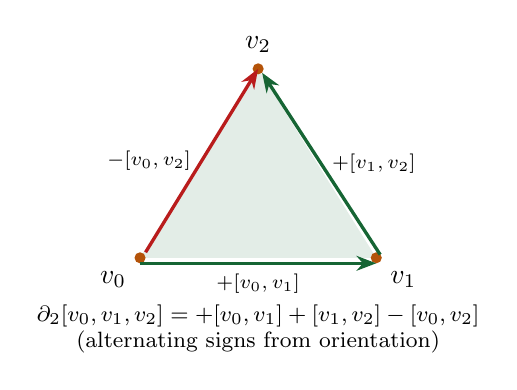
\begin{tikzpicture}[scale=1.0,
    vertex/.style={circle, fill=accent1, inner sep=0pt, minimum size=4pt},
    edgeplus/.style={draw=accent3, line width=1.2pt, -{Stealth[length=2.5mm]}},
    edgeminus/.style={draw=accent5, line width=1.2pt, -{Stealth[length=2.5mm]}}]
  \fill[accent3!12] (0,0) -- (3,0) -- (1.5, 2.4) -- cycle;
  \node[vertex, label=below left:{$v_0$}]  at (0,0) {};
  \node[vertex, label=below right:{$v_1$}] at (3,0) {};
  \node[vertex, label=above:{$v_2$}]       at (1.5, 2.4) {};
  \draw[edgeplus] (0,-0.07) -- (3,-0.07) node[midway, below, font=\scriptsize] {$+[v_0,v_1]$};
  \draw[edgeplus] (3.05, 0.04) -- (1.55, 2.35) node[midway, right, font=\scriptsize] {$+[v_1, v_2]$};
  \draw[edgeminus] (0.07, 0.07) -- (1.5, 2.4) node[midway, left, font=\scriptsize] {$-[v_0, v_2]$};
  \node[font=\footnotesize, align=center] at (1.5, -0.9)
    {$\partial_2 [v_0, v_1, v_2] = +[v_0, v_1] + [v_1, v_2] - [v_0, v_2]$\\
     (alternating signs from orientation)};
\end{tikzpicture}
\end{center}

\subsection{The fundamental identity}

\begin{theorem}[$\partial \circ \partial = 0$]
For any $k$, $\partial_{k-1} \circ \partial_k = 0$. Equivalently, the
image of $\partial_k$ is contained in the kernel of $\partial_{k-1}$.
\end{theorem}

This is the cornerstone of homology. The boundary of a boundary is
zero: the perimeter of a triangle, viewed as a chain of edges, has
zero net boundary because each vertex appears once with $+1$ and once
with $-1$. This identity is what makes the Hodge Laplacian well-defined.

\paragraph{Architectural use.} In G\"ombSoma the signed boundary
$\partial_2$ takes signed triangles to signed edges and is the
algebraic backbone of the Cartwright--Harary balance gate: a
triangle's $\sig$-product is $+1$ iff its boundary (as a chain) is
"trivial" in the appropriate quotient.

\section{Hodge Laplacian}

\begin{definition}[Hodge Laplacian at dimension $k$]
\[
\Delta_k = \partial_{k+1} \partial_{k+1}^* + \partial_k^* \partial_k
\]
where $\partial^*$ is the transpose (the \emph{coboundary} or
\emph{adjoint boundary} operator).
\end{definition}

The familiar graph Laplacian $\Delta_0 = D - A$ is precisely $\Delta_k$
at $k = 0$. The novelty at higher $k$:

\begin{itemize}
\item $\Delta_0$ acts on \emph{vertex} feature vectors. The standard
  graph Laplacian.
\item $\Delta_1$ acts on \emph{edge} feature vectors. Captures edge-flow
  dynamics; vortices and gradients are visible in its spectrum.
\item $\Delta_2$ acts on \emph{triangle} feature vectors. Captures
  face-flow; relevant when the data has well-defined $2$-simplices.
\end{itemize}

\begin{center}
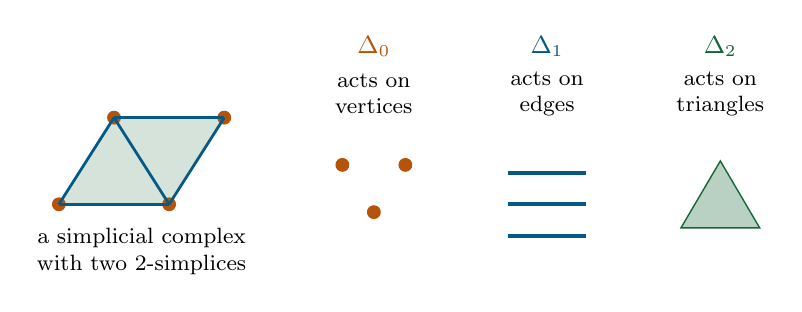
\begin{tikzpicture}[scale=1.0,
    vertex/.style={circle, fill=accent1, inner sep=0pt, minimum size=5pt},
    edge/.style={draw=accent2, line width=1.0pt},
    face/.style={fill=accent3!18, draw=accent3, line width=0.5pt}]
  % Sketch: a small 2-complex with the three Laplacians' "support"
  \begin{scope}
    \fill[face] (0,0) -- (1.4, 0) -- (0.7, 1.1) -- cycle;
    \fill[face] (1.4, 0) -- (2.1, 1.1) -- (0.7, 1.1) -- cycle;
    \node[vertex] at (0,0) {};
    \node[vertex] at (1.4, 0) {};
    \node[vertex] at (0.7, 1.1) {};
    \node[vertex] at (2.1, 1.1) {};
    \draw[edge] (0,0) -- (1.4,0);
    \draw[edge] (0,0) -- (0.7, 1.1);
    \draw[edge] (1.4, 0) -- (0.7, 1.1);
    \draw[edge] (1.4, 0) -- (2.1, 1.1);
    \draw[edge] (0.7, 1.1) -- (2.1, 1.1);
    \node[font=\footnotesize, align=center] at (1.05, -0.6)
      {a simplicial complex\\with two $2$-simplices};
  \end{scope}
  \begin{scope}[xshift=4.0cm]
    \node[font=\bfseries\small\color{accent1}] at (0, 2.0) {$\Delta_0$};
    \node[font=\footnotesize, align=center] at (0, 1.4) {acts on\\vertices};
    \node[vertex, fill=accent1] at (-0.4, 0.5) {};
    \node[vertex, fill=accent1] at (0.4, 0.5) {};
    \node[vertex, fill=accent1] at (0, -0.1) {};
  \end{scope}
  \begin{scope}[xshift=6.2cm]
    \node[font=\bfseries\small\color{accent2}] at (0, 2.0) {$\Delta_1$};
    \node[font=\footnotesize, align=center] at (0, 1.4) {acts on\\edges};
    \draw[edge, line width=1.5pt] (-0.5, 0.4) -- (0.5, 0.4);
    \draw[edge, line width=1.5pt] (-0.5, 0.0) -- (0.5, 0.0);
    \draw[edge, line width=1.5pt] (-0.5, -0.4) -- (0.5, -0.4);
  \end{scope}
  \begin{scope}[xshift=8.4cm]
    \node[font=\bfseries\small\color{accent3}] at (0, 2.0) {$\Delta_2$};
    \node[font=\footnotesize, align=center] at (0, 1.4) {acts on\\triangles};
    \fill[face, fill=accent3!30] (-0.5,-0.3) -- (0.5,-0.3) -- (0,0.55) -- cycle;
  \end{scope}
\end{tikzpicture}
\end{center}

\subsection{Hodge decomposition}

\begin{theorem}[Hodge decomposition]
Any $k$-chain $\omega$ decomposes uniquely as
\[
\omega = \omega_{\rm harm} \;+\; \partial_{k+1} \alpha \;+\; \partial_k^* \beta
\]
where $\omega_{\rm harm} \in \ker \Delta_k$ is \emph{harmonic},
$\partial_{k+1} \alpha$ is a \emph{boundary} (``curl-free'' analogue),
and $\partial_k^* \beta$ is a \emph{coboundary}
(``gradient'' analogue).
\end{theorem}

The harmonic part is the topologically invariant content. Its
dimension is the $k$-th Betti number $\beta_k$ --- a count of
$k$-dimensional ``holes'' in the complex. For a connected graph,
$\beta_0 = 1$ (one connected component); $\beta_1$ counts independent
cycles.

\paragraph{Architectural use.} In G\"ombSoma the harmonic part of a
vertex feature field captures features that survive a heat-flow
smoothing (next section); these are the ``topologically protected''
features at the input scale.

\section{Heat kernel}

The heat equation on the simplicial complex is
\[
\partial_t \omega_t = -\Delta_k \omega_t,
\qquad \omega_0 = f,
\]
with solution $\omega_t = \exp(-t \Delta_k) f$. The operator
$\exp(-t \Delta_k)$ is the \emph{heat kernel}; it smooths features at
spatial scale $\sqrt{t}$.

\begin{center}
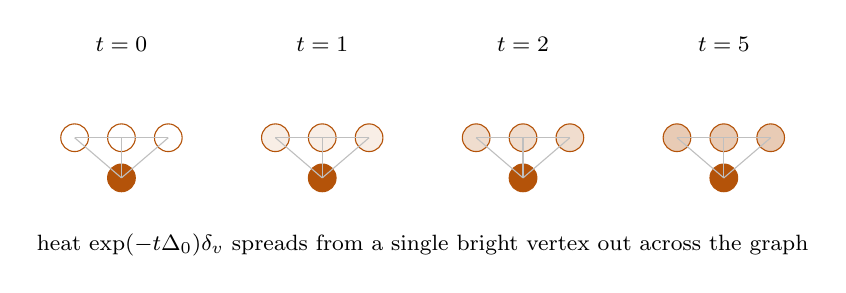
\begin{tikzpicture}[scale=0.85,
    vertex/.style={circle, draw=accent1, inner sep=0pt, minimum size=10pt}]
  \foreach \t/\x/\dot in {{0}/0/0, {1}/3/1, {2}/6/2, {5}/9/3} {
    \begin{scope}[xshift=\x cm]
      \node[font=\footnotesize\bfseries] at (0, 2.0) {$t = \t$};
      \node[vertex, fill=accent1!\dot 0] at (-0.7, 0.6) {};
      \node[vertex, fill=accent1!\dot 0] at ( 0.0, 0.6) {};
      \node[vertex, fill=accent1!\dot 0] at ( 0.7, 0.6) {};
      \node[vertex, fill=accent1] at (0.0, -0.0) {};
      \draw[draw=gray!50] (-0.7, 0.6) -- (0.0, -0.0);
      \draw[draw=gray!50] ( 0.0, 0.6) -- (0.0, -0.0);
      \draw[draw=gray!50] ( 0.7, 0.6) -- (0.0, -0.0);
      \draw[draw=gray!50] (-0.7, 0.6) -- ( 0.0, 0.6);
      \draw[draw=gray!50] ( 0.0, 0.6) -- ( 0.7, 0.6);
    \end{scope}
  }
  \node[font=\footnotesize, align=center] at (4.5, -1.0)
    {heat $\exp(-t \Delta_0) \delta_v$ spreads from a single bright vertex out across the graph};
\end{tikzpicture}
\end{center}

\paragraph{Architectural use.} In G\"ombSoma the \emph{Hodge term} in
the Bochner-coupled message passing
($\alpha \cdot (\Delta_k h)_c$) is one explicit step of heat diffusion;
the layer learns to interpolate between flat connection
(no smoothing), Hodge smoothing (continuous), and Ricci correction
(geometric).

\section{Forman-Ricci curvature}

\begin{definition}[Forman-Ricci $\kappa(e)$, unweighted]
For an edge $e = (u, v)$ in a simplicial complex,
\[
\kappa(e) = 2 - \deg(u) - \deg(v) + 2 \cdot |\Delta(u, v)|
\]
where $|\Delta(u, v)|$ is the number of triangles incident on $e$.
\end{definition}

\paragraph{Reading the formula.}
\begin{itemize}
\item Each triangle adds $+2$ (a face filling the corner around $e$).
\item Each degree adds $-1$ per incident neighbour (edge is being
  stretched between busy hubs).
\item The leading $+2$ is the "flat-space" constant.
\end{itemize}

Complete graphs $K_n$ achieve $\kappa = 0$ everywhere
(triangle-balanced); cycles $C_n$ ($n \geq 4$) achieve
$\kappa = -2$ everywhere (no triangles, deg 2 + 2). Stars $S_n$ give
strongly negative $\kappa = 1 - n$ (severe bottleneck).

\begin{center}
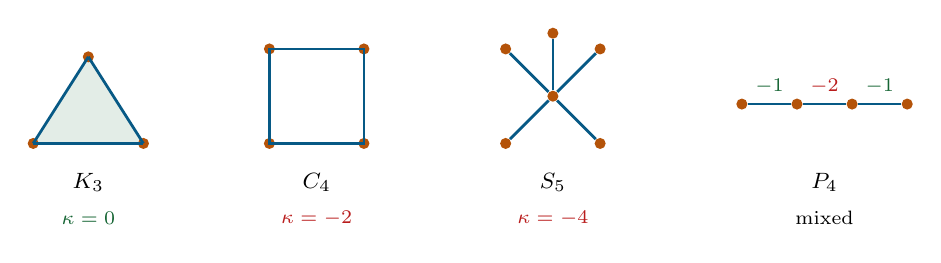
\begin{tikzpicture}[scale=1.0,
    vertex/.style={circle, fill=accent1, inner sep=0pt, minimum size=4pt},
    edge/.style={draw=accent2, line width=1.0pt}]
  % K3 -- $\kappa$ = 0
  \begin{scope}
    \fill[accent3!12] (0,0) -- (1.4, 0) -- (0.7, 1.1) -- cycle;
    \node[vertex] at (0,0) {};
    \node[vertex] at (1.4, 0) {};
    \node[vertex] at (0.7, 1.1) {};
    \draw[edge] (0,0) -- (1.4, 0);
    \draw[edge] (1.4, 0) -- (0.7, 1.1);
    \draw[edge] (0, 0) -- (0.7, 1.1);
    \node[font=\footnotesize\bfseries] at (0.7, -0.5) {$K_3$};
    \node[font=\scriptsize\color{accent3}] at (0.7, -0.95) {$\kappa = 0$};
  \end{scope}
  % C4 -- $\kappa$ = -2
  \begin{scope}[xshift=3.0cm]
    \node[vertex] at (0,0) {};
    \node[vertex] at (1.2, 0) {};
    \node[vertex] at (1.2, 1.2) {};
    \node[vertex] at (0, 1.2) {};
    \draw[edge] (0,0) -- (1.2, 0) -- (1.2, 1.2) -- (0, 1.2) -- cycle;
    \node[font=\footnotesize\bfseries] at (0.6, -0.5) {$C_4$};
    \node[font=\scriptsize\color{accent5}] at (0.6, -0.95) {$\kappa = -2$};
  \end{scope}
  % Star S_5 -- $\kappa$ = -4
  \begin{scope}[xshift=6.0cm]
    \node[vertex] (c) at (0.6, 0.6) {};
    \node[vertex] (l1) at (0, 0) {};
    \node[vertex] (l2) at (1.2, 0) {};
    \node[vertex] (l3) at (1.2, 1.2) {};
    \node[vertex] (l4) at (0, 1.2) {};
    \node[vertex] (l5) at (0.6, 1.4) {};
    \draw[edge] (c) -- (l1);
    \draw[edge] (c) -- (l2);
    \draw[edge] (c) -- (l3);
    \draw[edge] (c) -- (l4);
    \draw[edge] (c) -- (l5);
    \node[font=\footnotesize\bfseries] at (0.6, -0.5) {$S_5$};
    \node[font=\scriptsize\color{accent5}] at (0.6, -0.95) {$\kappa = -4$};
  \end{scope}
  % Path P4 -- $\kappa$ = -1, -2, -1
  \begin{scope}[xshift=9.0cm]
    \node[vertex] (a) at (0,0.5) {};
    \node[vertex] (b) at (0.7, 0.5) {};
    \node[vertex] (e) at (1.4, 0.5) {};
    \node[vertex] (d) at (2.1, 0.5) {};
    \draw[edge] (a) -- node[above, font=\scriptsize\color{accent3}] {$-1$} (b);
    \draw[edge] (b) -- node[above, font=\scriptsize\color{accent5}] {$-2$} (e);
    \draw[edge] (e) -- node[above, font=\scriptsize\color{accent3}] {$-1$} (d);
    \node[font=\footnotesize\bfseries] at (1.05, -0.5) {$P_4$};
    \node[font=\scriptsize] at (1.05, -0.95) {mixed};
  \end{scope}
\end{tikzpicture}
\end{center}

\paragraph{The diagnostic.} Strongly negative $\kappa$ marks
\emph{bottlenecks}: edges over which information must pass but which
are stretched thin. Topping et al.\ \cite{Topping2022} showed that
GNNs over graphs with strongly negative-$\kappa$ edges exhibit
\emph{exponential} feature compression --- the over-squashing problem.
Their solution, SDRF (Section \ref{sec:sdrf}), iteratively rewires the
graph to lift $\min_e \kappa(e)$.

\paragraph{Architectural use.} In G\"ombSoma:
\begin{itemize}
\item Phase 2's \texttt{AdaptiveQuadtree} subdivides anchors with
  high $|\kappa_v|$ --- pushing the bottleneck signal as a
  scale-refinement criterion.
\item Phase 4's Bochner-coupled \texttt{HypergraphConv} adds a
  $\kappa$-weighted correction term to each message-passing step.
\item Phase 6's SDRF rewiring adds shortcut edges where $\kappa$ is
  too negative.
\end{itemize}

\section{Ollivier-Ricci curvature (a contrast)}

For comparison, Ollivier-Ricci $\kappa_{\rm O}$ is defined via
optimal transport:
\[
\kappa_{\rm O}(u, v) = 1 - \frac{W_1(\mu_u, \mu_v)}{d(u, v)},
\]
where $\mu_u$ is a probability measure on $u$'s neighbourhood (often
uniform on $N(u)$) and $W_1$ is the $1$-Wasserstein distance.

\paragraph{Why Forman instead.} $W_1$ requires solving a linear-
programming problem per edge --- prohibitively expensive at the
per-layer scale we need. Forman is purely combinatorial: degree
counts and triangle counts, computable in $O(|E| \cdot \bar d)$.
Practically: Forman per layer, Ollivier reserved for post-hoc
analysis if needed.

\section{Bochner--Weitzenböck identity}

In smooth Riemannian geometry, the Hodge Laplacian on $1$-forms
factors as
\[
\Delta_1 \omega \;=\; \nabla^* \nabla \omega \;+\; \mathrm{Ric}(\omega^\sharp)^\flat,
\]
which decomposes the Laplacian into a \emph{flat connection} term
$\nabla^* \nabla$ (ordinary smoothing) and a \emph{Ricci correction}
term that bends the smoothing in directions of high curvature.

On a discrete simplicial complex the identity carries over with
$\nabla^* \nabla$ replaced by the \emph{vertex-incidence Laplacian}
and $\mathrm{Ric}$ replaced by the Forman correction. This is
exactly what we exploit in G\"ombSoma's Phase 4 Bochner-coupled
\texttt{HypergraphConv}:
\[
\text{msg}(c) = \psi_{\pi(c)} \Bigl(
   \underbrace{\sum_i W_i x_{v_i}}_{\text{flat}}
   + \alpha \cdot \underbrace{(\Delta_k h)_c}_{\text{Hodge}}
   + \beta \cdot \underbrace{\sum_i \kappa(e_i) W_i x_{v_i}}_{\text{Ricci correction}}
\Bigr).
\]
With $\alpha = \beta = 0$ the layer reproduces a vanilla
message-pass. Increasing $\alpha$ adds heat-kernel smoothing; increasing
$\beta$ adds the curvature correction. The Bochner identity says
these two terms are not arbitrary --- they are the natural
decomposition of the underlying geometric Laplacian.

\section{Discrete Ricci flow and SDRF}\label{sec:sdrf}

\emph{Ricci flow} on a smooth manifold deforms the metric in the
direction of negative Ricci curvature:
$\partial_t g_{ij} = -2 \mathrm{Ric}_{ij}$. Hamilton (1982) introduced it;
Perelman used it to prove the Poincaré conjecture (2003).

\paragraph{Discrete analogue (SDRF, \cite{Topping2022}).} For each
strongly-negative-$\kappa$ edge in a graph, add a shortcut edge
between unrelated neighbours of its endpoints. Iterate. The result
is a graph with $\min_e \kappa(e)$ bounded away from $-\infty$ ---
\emph{the over-squashing bottleneck has been relieved}.

\begin{center}
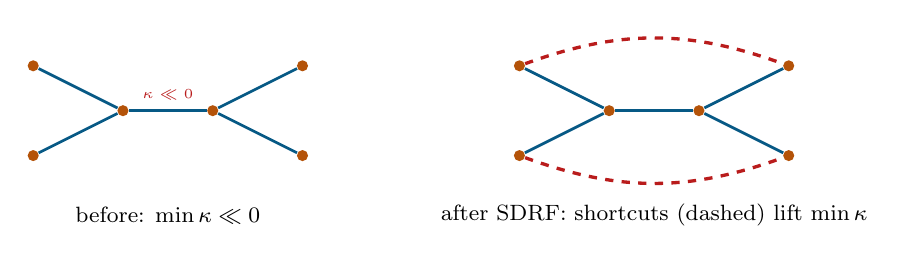
\begin{tikzpicture}[scale=0.95,
    vertex/.style={circle, fill=accent1, inner sep=0pt, minimum size=4pt},
    edge/.style={draw=accent2, line width=1.0pt},
    rewired/.style={draw=accent5, line width=1.2pt, dashed}]
  % Before: bottleneck path
  \begin{scope}
    \node[vertex] (a1) at (0, 0.6) {};
    \node[vertex] (a2) at (0, -0.6) {};
    \node[vertex] (m1) at (1.2, 0) {};
    \node[vertex] (m2) at (2.4, 0) {};
    \node[vertex] (b1) at (3.6, 0.6) {};
    \node[vertex] (b2) at (3.6, -0.6) {};
    \draw[edge] (a1) -- (m1) -- (a2);
    \draw[edge] (m1) -- node[above, font=\tiny\color{accent5}] {$\kappa \ll 0$} (m2);
    \draw[edge] (m2) -- (b1);
    \draw[edge] (m2) -- (b2);
    \node[font=\footnotesize, align=center] at (1.8, -1.4)
      {before: $\min \kappa \ll 0$};
  \end{scope}
  \begin{scope}[xshift=6.5cm]
    \node[vertex] (a1) at (0, 0.6) {};
    \node[vertex] (a2) at (0, -0.6) {};
    \node[vertex] (m1) at (1.2, 0) {};
    \node[vertex] (m2) at (2.4, 0) {};
    \node[vertex] (b1) at (3.6, 0.6) {};
    \node[vertex] (b2) at (3.6, -0.6) {};
    \draw[edge] (a1) -- (m1) -- (a2);
    \draw[edge] (m1) -- (m2);
    \draw[edge] (m2) -- (b1);
    \draw[edge] (m2) -- (b2);
    \draw[rewired] (a1) to[out=20,in=160] (b1);
    \draw[rewired] (a2) to[out=-20,in=200] (b2);
    \node[font=\footnotesize, align=center] at (1.8, -1.4)
      {after SDRF: shortcuts (dashed) lift $\min \kappa$};
  \end{scope}
\end{tikzpicture}
\end{center}

\paragraph{Architectural use.} Phase 6 of Ricci-Stim applies SDRF once
to the multi-scale patch hypergraph before message passing; this is
the principled answer to ``our graph has a bottleneck through every
patch in the 4-connected interior.''

\section{Discrete Gauss--Bonnet (brief)}

For a closed simply-connected planar region of a simplicial complex,
\[
\sum_v K_v \;=\; \chi
\]
where $K_v$ is a suitable \emph{vertex curvature} and $\chi$ is the
Euler characteristic of the region. The full identity using Forman
$\kappa$ involves face contributions; on the unit tests we settle for
the simpler combinatorial check $\sum_e \kappa(e)$ on small examples.

\paragraph{Architectural use.} Sanity check that the Forman $\kappa$
computation is correct (Phase 1 unit test).

\section{Putting it all together --- the architecture in one diagram}

\begin{center}
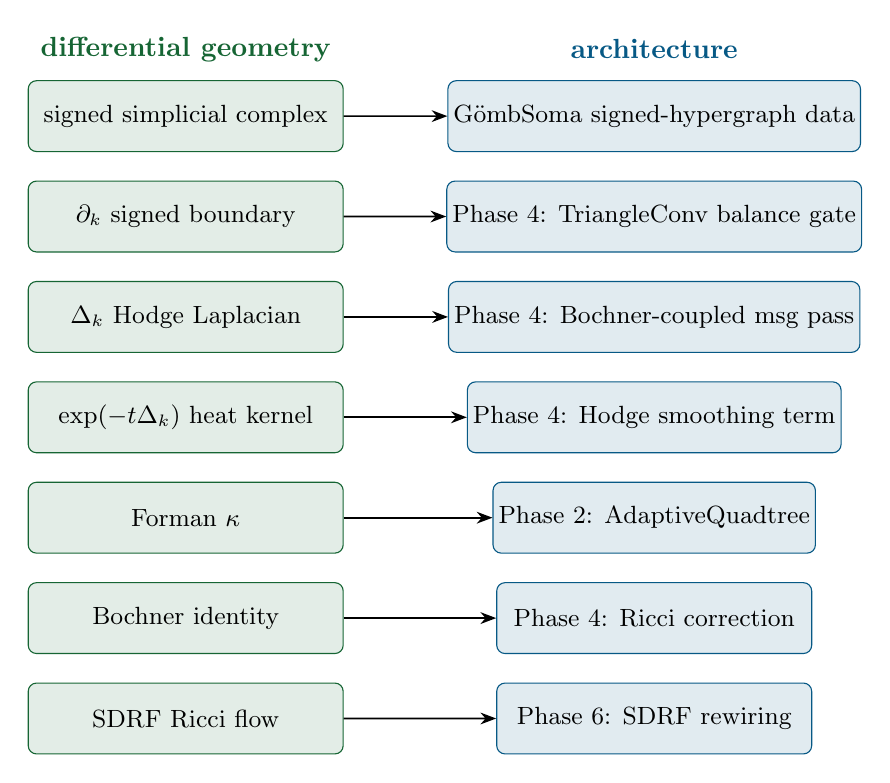
\begin{tikzpicture}[scale=0.85,
    box/.style={draw, rounded corners=3pt, minimum width=4.0cm,
                minimum height=9mm, align=center, font=\small, inner sep=2pt},
    dgbox/.style={box, fill=accent3!12, draw=accent3},
    archbox/.style={box, fill=accent2!12, draw=accent2},
    arr/.style={-{Stealth[length=2mm]}, line width=0.6pt}]
  \node[dgbox]   (sc)  at (-3, 5.5) {signed simplicial complex};
  \node[dgbox]   (bd)  at (-3, 4.0) {$\partial_k$ signed boundary};
  \node[dgbox]   (hl)  at (-3, 2.5) {$\Delta_k$ Hodge Laplacian};
  \node[dgbox]   (hk)  at (-3, 1.0) {$\exp(-t\Delta_k)$ heat kernel};
  \node[dgbox]   (fr)  at (-3,-0.5) {Forman $\kappa$};
  \node[dgbox]   (bo)  at (-3,-2.0) {Bochner identity};
  \node[dgbox]   (sd)  at (-3,-3.5) {SDRF Ricci flow};

  \node[archbox] (gs)  at ( 4, 5.5) {G\"ombSoma signed-hypergraph data};
  \node[archbox] (pol) at ( 4, 4.0) {Phase 4: TriangleConv balance gate};
  \node[archbox] (msg) at ( 4, 2.5) {Phase 4: Bochner-coupled msg pass};
  \node[archbox] (smt) at ( 4, 1.0) {Phase 4: Hodge smoothing term};
  \node[archbox] (qt)  at ( 4,-0.5) {Phase 2: AdaptiveQuadtree};
  \node[archbox] (boc) at ( 4,-2.0) {Phase 4: Ricci correction};
  \node[archbox] (re)  at ( 4,-3.5) {Phase 6: SDRF rewiring};

  \draw[arr] (sc)  -- (gs);
  \draw[arr] (bd)  -- (pol);
  \draw[arr] (hl)  -- (msg);
  \draw[arr] (hk)  -- (smt);
  \draw[arr] (fr)  -- (qt);
  \draw[arr] (bo)  -- (boc);
  \draw[arr] (sd)  -- (re);

  \node[font=\bfseries, color=accent3] at (-3, 6.5) {differential geometry};
  \node[font=\bfseries, color=accent2] at ( 4, 6.5) {architecture};
\end{tikzpicture}
\end{center}

\section{Further reading}

\begin{thebibliography}{99}

\bibitem{Forman2003}
R. Forman, ``Bochner's Method for Cell Complexes and Combinatorial
Ricci Curvature,'' \emph{Discrete \& Computational Geometry},
vol.~29, no.~3, pp.~323--374, 2003.

\bibitem{Topping2022}
J. Topping, F. Di Giovanni, B. P. Chamberlain, X. Dong, M. M.
Bronstein, ``Understanding Over-Squashing and Bottlenecks on Graphs
via Curvature,'' \emph{ICLR}, 2022.\\
\texttt{arXiv:2111.14522}

\bibitem{Cartwright1956}
D. Cartwright, F. Harary, ``Structural Balance: A Generalization of
Heider's Theory,'' \emph{Psychological Review}, vol.~63, no.~5,
pp.~277--293, 1956.

\bibitem{Ollivier2009}
Y. Ollivier, ``Ricci curvature of Markov chains on metric spaces,''
\emph{Journal of Functional Analysis}, vol.~256, no.~3,
pp.~810--864, 2009.

\bibitem{Lim2020}
L.-H. Lim, ``Hodge Laplacians on Graphs,'' \emph{SIAM Review},
vol.~62, no.~3, pp.~685--715, 2020.

\bibitem{Bodnar2021}
C. Bodnar, F. Frasca, et al., ``Weisfeiler and Lehman Go Topological:
Message Passing Simplicial Networks,'' \emph{ICML}, 2021.

\bibitem{Hansen2020}
J. Hansen, T. Gebhart, ``Sheaf Neural Networks,'' \emph{NeurIPS-W},
2020.

\bibitem{Knill2010}
O. Knill, ``A Discrete Gauss--Bonnet Type Theorem,''
\emph{Elemente der Mathematik}, vol.~67, no.~1, pp.~1--17, 2012.

\bibitem{Bochner1946}
S. Bochner, ``Vector Fields and Ricci Curvature,'' \emph{Bulletin of
the American Mathematical Society}, vol.~52, no.~9,
pp.~776--797, 1946.

\bibitem{Bronstein2021}
M. M. Bronstein, J. Bruna, T. Cohen, P. Veličković,
``Geometric Deep Learning: Grids, Groups, Graphs, Geodesics, and
Gauges,'' Pre-print, 2021.\\
\texttt{arXiv:2104.13478}

\end{thebibliography}

\section{One-line takeaways}

\begin{center}
\begin{tabular}{lp{10cm}}
\toprule
Concept & One-line takeaway for G\"ombSoma\\
\midrule
Simplicial complex     & vertices + edges + triangles + \ldots; the natural home of signed hypergraphs \\
Signed boundary $\partial_k$ & alternating-sign map between simplex dimensions; the algebraic backbone of cycles \\
$\partial \circ \partial = 0$ & boundary-of-boundary vanishes; makes the Hodge Laplacian well-defined \\
Hodge Laplacian $\Delta_k$ & per-dimension diffusion operator; harmonic kernel = topology-invariant features \\
Hodge decomposition    & every feature = harmonic + gradient + curl \\
Heat kernel $\exp(-t\Delta_k)$ & smoothing at spatial scale $\sqrt{t}$; the natural generalisation of Gaussian blur \\
Forman $\kappa(e)$     & combinatorial Ricci: positive = clique, negative = bottleneck \\
Ollivier $\kappa_{\rm O}$ & optimal-transport Ricci; rigorous but expensive \\
Bochner--Weitzenböck   & $\Delta_1 = \nabla^* \nabla + \mathrm{Ric}$; the principled message-pass decomposition \\
SDRF Ricci flow        & graph-rewiring to remove bottlenecks; addresses over-squashing \\
Discrete Gauss--Bonnet & $\sum \kappa = \chi$ on closed regions; a Forman sanity check \\
\bottomrule
\end{tabular}
\end{center}

\vspace{1em}
\hrule height 0.4pt
\vspace{0.5em}
\emph{End of primer.}

\end{document}
